\chapter{Pruebas de escala}

% **************************** Define Graphics Path **************************
\graphicspath{{Chapter4/Figs/}}

Con el entorno de simulación construido, el siguiente objetivo es realizar pruebas de escala sobre la arquitectura. Se realizan dos tipos de pruebas de escala: (a) verificar cómo funciona la arquitectura para topologias de escala, (b) realizar estudios de escala sobre la cantidad de servicios. En este capítulo se explicará el propósito de cada prueba, las condiciones bajo las cuales se ejecuta cada una de ellas (topologias, tipos de tráfico, etc) y por último, los resultados que arrojan. Todas las pruebas fueron realizadas en una máquina virtual con 32GB de RAM, procesador X y Lubuntu 14.04 como sistema operativo.

\section{Topologias de escala}
Es importante poder asegurar que la arquitectura puede ser fácilmente migrada a redes reales. Para poder asegurar esto, se diseñan los dos siguientes escenarios de prueba. El primero consiste en verificar los aspectos críticos de la arquitectura, como el algoritmo de ruteo y la clasificación de tráfico. En el segundo escenario se intenta estudiar como impacta el largo del camino y las características de la topología sobre el tiempo que demora el controlador en dar de alta una red privada virtual. Ambos escenarios utilizan un conjunto de topologias de prueba, que se listan a continuación:
\begin{itemize}
	\item \textbf{Básica}: 4 nodos en topología de full mesh. Es la utilizada en el prototipo físico. Figura \ref{fig:topo_basica}.
	\item \textbf{Chica}: topología arbitraria de 11 nodos (fuente: Topology Zoo). Figura \ref{fig:topo_chica}.
	\item \textbf{Mediana}: topología arbitraria de 45 nodos (fuente: Topology Zoo). Figura \ref{fig:topo_mediana}.
	\item \textbf{Grande}: topología de tipo arborescente compuesta por 105 nodos. Figura \ref{fig:topo_grande}
\end{itemize}

Todas las topologias tienen las siguientes características:
\begin{itemize}
	\item Tienen un conjunto de RAUSwitch, conectados de acuerdo a lo que dicte la topología.
	\item Existen dos subredes cliente, implementadas por un QuaggaRouter y un RAUHost cada una (recordar las clases del entorno virtual). El RAUHost representa la computadora que utiliza el usuario final para conectarse a la red, y QuaggaRouter representa el router legacy que conecta la subred del usuario a la red SDN. Los RAUHost serán los remitentes y destinatarios del tráfico que pasará por la red. Esos datos se generarán con el comando \textit{ping} y la herramienta \textit{iperf}. Estas dos subredes tendrán una ubicación variable en cada topología, ya que se probará con distintos caminos entre ellas. Por esta razón, se omiten en las imágenes de las topologias.
	\item El controlador se conecta con un switch virtual genérico (gracias a la clase Switch de Mininet, en el modo \textit{standalone}), que a su vez se conectará con los RAUSwitch. Esta será la red de gestión. Por simplicidad, dicha red se omite en las imágenes.
\end{itemize}

\begin{figure}[t]
	\caption{Topología básica}
	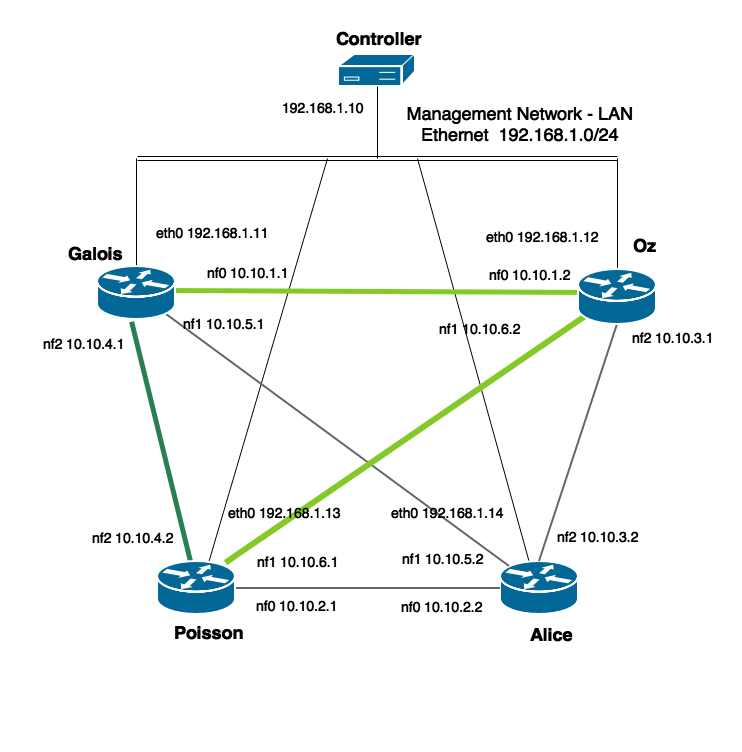
\includegraphics[scale=0.4]{topo_basica}
	\centering
	\label{fig:topo_basica}
\end{figure}

\begin{figure}[t]
	\caption{Topología chica}
	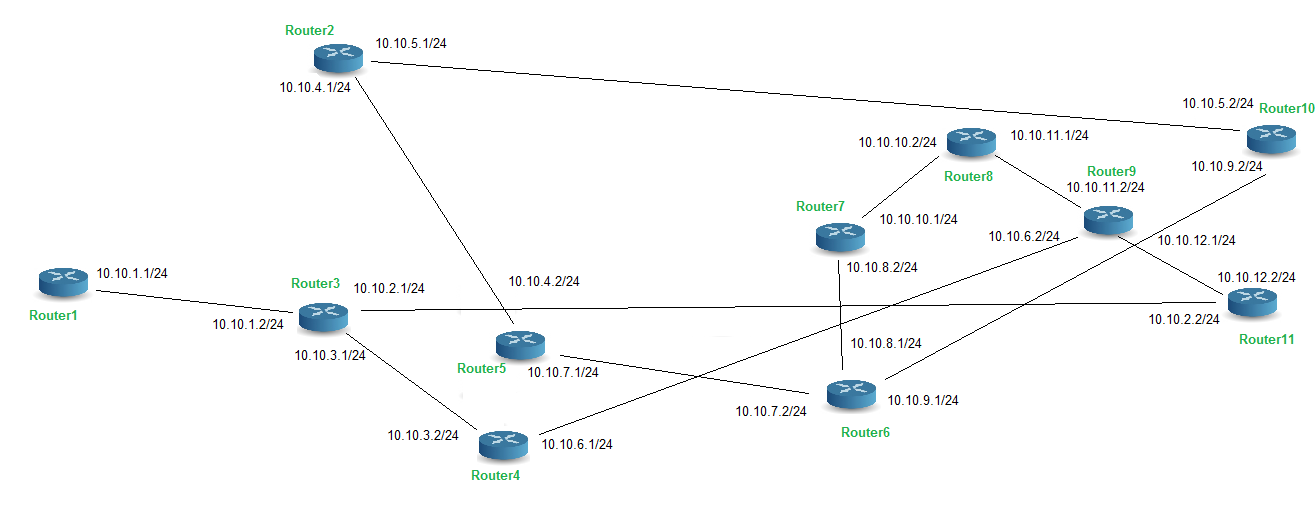
\includegraphics[scale=0.4]{topo_chica}
	\centering
	\label{fig:topo_chica}
\end{figure}

\begin{figure}[t]
	\caption{Topología mediana}
	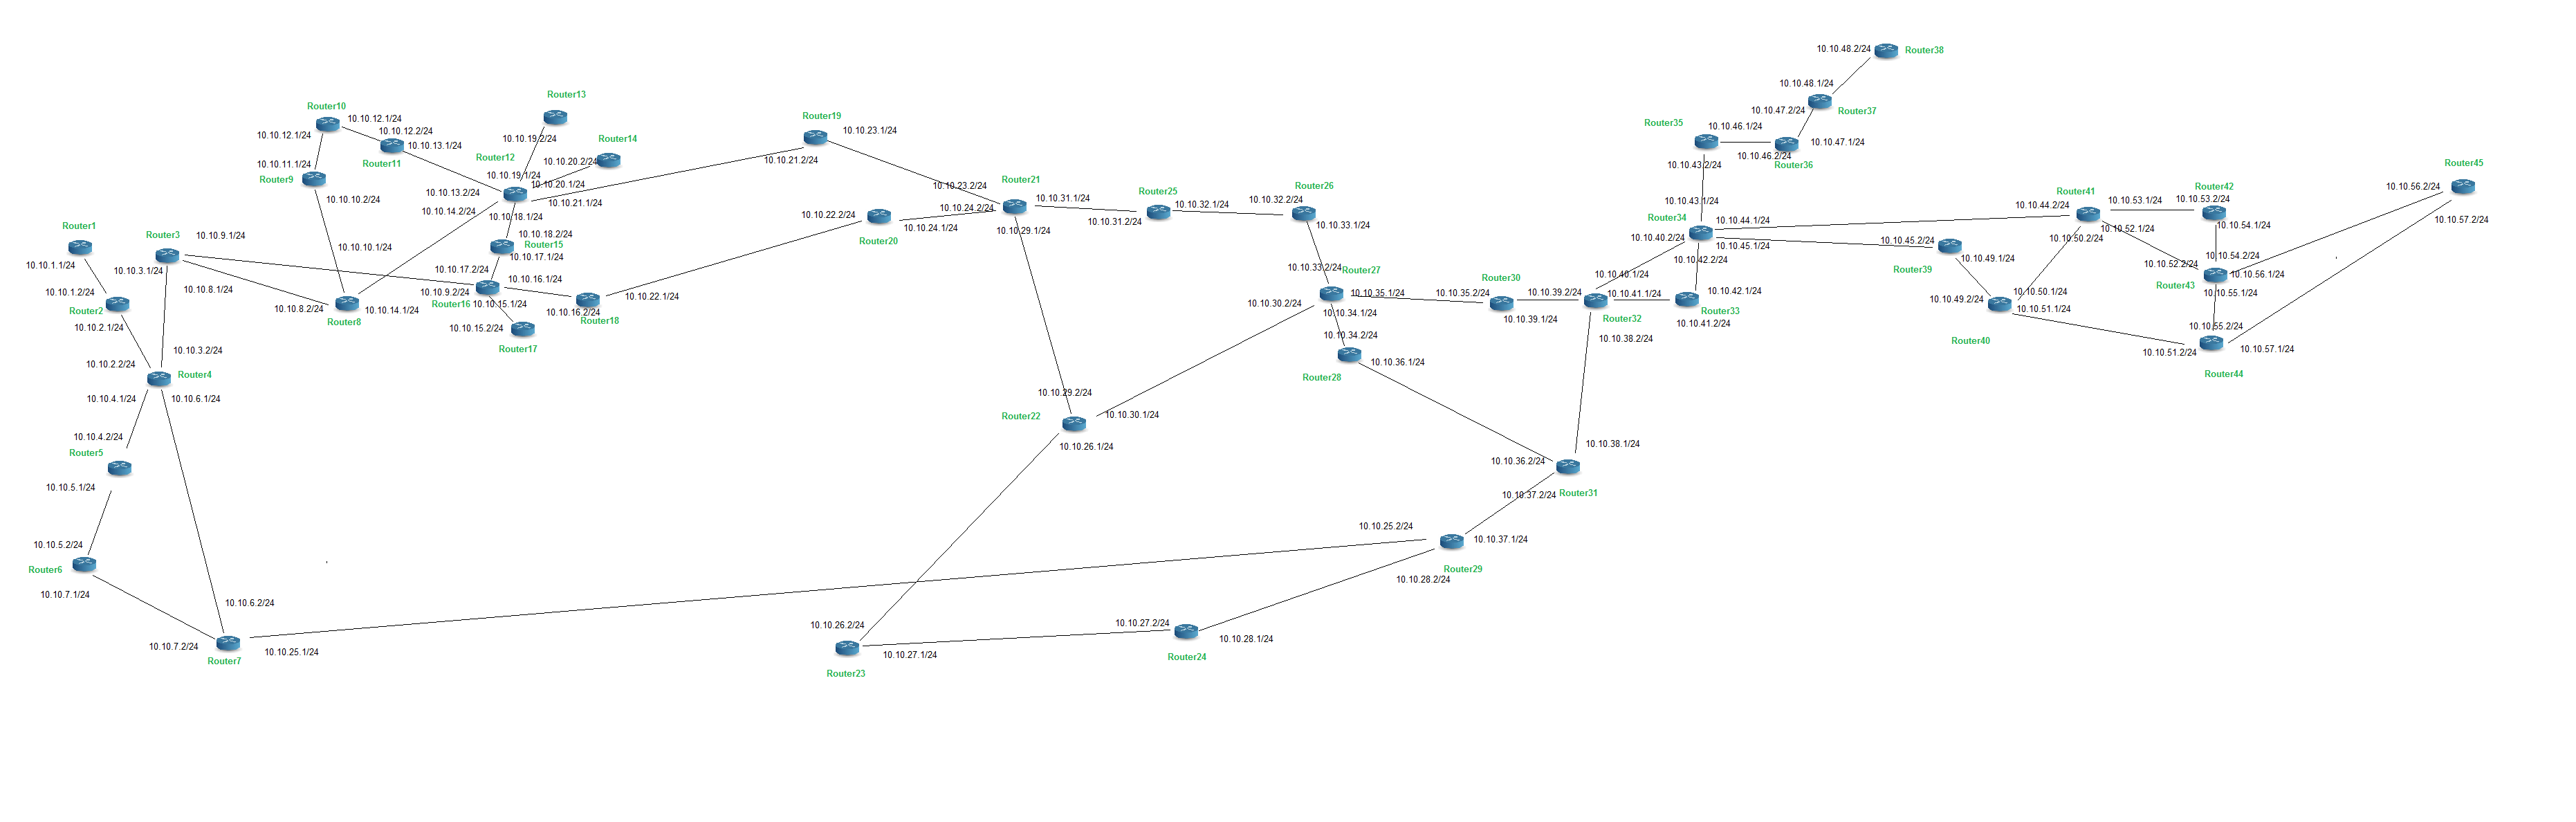
\includegraphics[width=\textwidth,height=\textheight,keepaspectratio]{topo_mediana}
	\centering
	\label{fig:topo_mediana}
\end{figure}

\begin{figure}[t]
	\caption{Topología grande}
	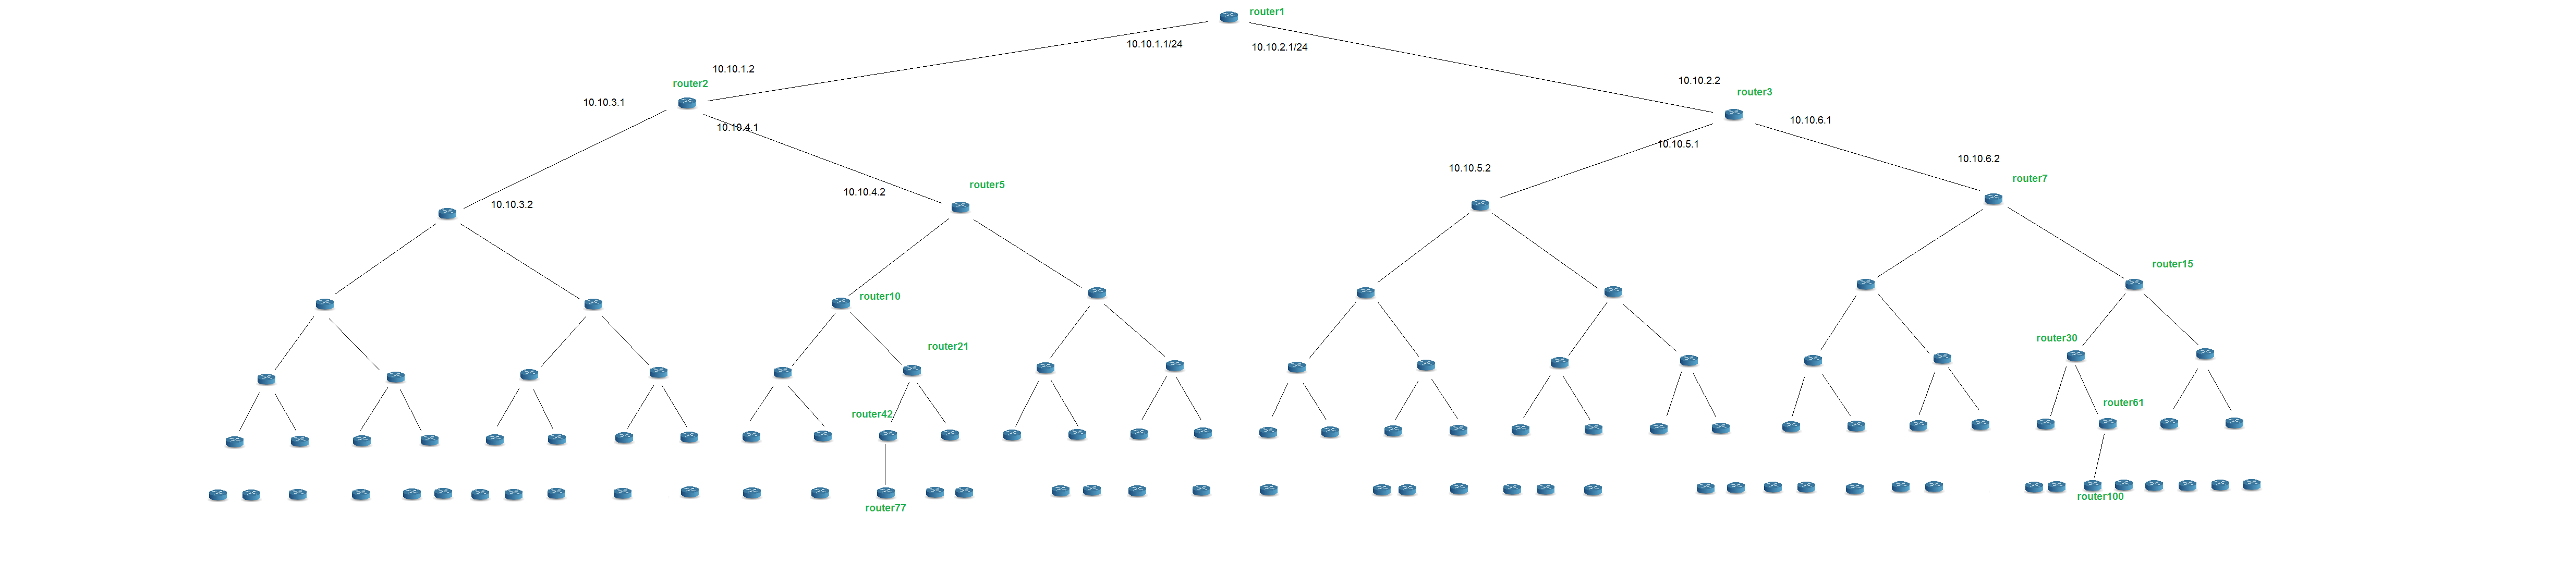
\includegraphics[width=\textwidth,height=\textheight,keepaspectratio]{topo_grande}
	\centering
	\label{fig:topo_grande}
\end{figure}

\subsection{Escenario 1}
En este escenario se crea una VPN punto a punto de capa 3 entre las dos subredes cliente, y se controla que tanto la creación de la VPN como el uso de la misma con tráfico, funciona correctamente. Esto se repite para cada topología de prueba. Los puntos específicos que se busca verificar se detallan a continuación: \\ \\
\textbf{Algoritmo de ruteo} \\
Se verifican dos aspectos claves: que el camino se corresponde con el camino esperado (calculado previamente de forma manual), y que el camino es correctamente instalado en forma de reglas de reenvío (en base a conmutación de etiquetas MPLS) en las respectivas tablas de flujos OpenFlow de cada nodo del camino. Todo esto se puede comprobar analizando las tablas de flujos de cada nodo, que se pueden ver utilizando el comando \textbf{dump-flows} de Open vSwitch. También se puede utilizar la interfaz gráfica de RAUFlow, aunque no se recomienda su uso con topologias grandes (como pueden ser la mediana o grande, en este caso) ya que la forma de presentar los nodos se vuelve demasiado caótica. Desde las tablas de flujos se puede reconstruir el camino que computó la aplicación, y también comprobar que los flujos manipulan correctamente las etiquetas MPLS. \\ \\
\textbf{Clasificación de tráfico} \\
La idea es verificar que realmente se están asignando las etiquetas MPLS al tráfico entrante, así como comprobar que el mismo es reenviado por los nodos correctos. Para probar esto se utilizará una VPN de capa 3, que permitirá tráfico con ethertype 0x0800, es decir, del protocolo IPv4. Se generará tráfico de este tipo utilizando el comando \textbf{ping} y la herramienta \textbf{iperf}. Con la herramienta tcpdump, se verificará que el tráfico pasa correctamente por cada nodo del camino. \\

\begin{table}[ht]
	\caption{Pasos que cumple cada caso en la creación y uso exitoso de un servicio.}
	\centering 
	\resizebox{\textwidth}{!}{%
		\begin{tabular}{c c c c c}
			\hline\hline
			Largo del camino (topología) & Servicio & Camino & Flujos  & Clasificación de tráfico \\ [0.5ex]
			\hline
			1 (básica) & X & X & X & X \\
			7 (chica) & X & X &  &  \\
			10 (mediana) &  &  &  &  \\
			12 (grande) &  &  &  &  \\ [1ex]
			\hline
		\end{tabular}
	}
	\label{table:problemas_por_topologia}
\end{table}

Con el propósito de hacer un diagnóstico más preciso sobre el proceso de creación y uso de una VPN, se lo descompone de 4 pasos conceptuales en los cuales podría haber fallas. Estos pasos son: (a) se crea con éxito el servicio, (b) el camino que se calcula es correcto, (c) los flujos de cada nodo del camino son correctos, (d) se clasifica correctamente el tráfico. Si se cumplen los 3 primeros pasos quiere decir que el servicio (y por ende la VPN que lo utilice) se establece correctamente y si se cumple el último paso entonces el tráfico pasa sin problemas por el servicio creado. En la tabla \ref{table:problemas_por_topologia} se detallan los comportamientos observados para algunos de los casos estudiados. En ella se indica con una X los pasos que funcionaron correctamente para cada caso. Las celdas vacías indican qué paso falló en cada caso. \\

Analizando la tabla \ref{table:problemas_por_topologia} se pueden observar como mínimo dos problemas. El primero es que en el caso de la topología chica y un camino de 7 saltos, el servicio se crea y los flujos están en los nodos correctos (los del camino más corto entre las subredes cliente), pero los mismos no son correctos. El segundo comportamiento que se observa es que para el caso del camino de 10 saltos en la topología mediana, y el de 12 saltos en la topología grande, el servicio ni siquiera llega a crearse correctamente, es decir, la aplicación sufre una excepción de Python al intentar hacerlo. Las razones que explican esto, así como sus respectivas soluciones (si son posibles) se encuentran en la anterior sección 3.5, donde se explican los problemas encontrados y/o resueltos en el entorno. El resto de las pruebas que se mencionan en este capítulo fueron realizadas con dichas correcciones ya hechas.

\subsection{Escenario 2}
El objetivo de este escenario es estudiar como impacta el tamaño de la topología y el largo del camino en el tiempo que demora la arquitectura en establecer una VPN. Se espera que ese tiempo sea influenciado en gran medida por dos factores: el tiempo que demora el controlador en calcular el camino óptimo y el tiempo que demora en configurar los flujos en cada nodo. Dado que los servicios se crean enviando pedidos HTTP POST al controlador, el tiempo de creación de los mismos se medirá como el tiempo que demore el controlador en devolver las respuestas HTTP indicando que fueron creados con éxito (esta información está disponible en los logs). Para lograr resultados representativos y reducir el margen de error, en lugar de crear una VPN y medir su tiempo solamente, se realizan cuatro ejecuciones y se calculan las métricas estadísticas relevantes. Para agilizar la ejecución de esta prueba se utiliza un script en Python que manda los pedidos HTTP POST al controlador para crear las VPN, y de este modo no hay necesidad de hacerlo manualmente a través de la interfaz web.
\begin{table}[!h]
	\caption{Tiempo de demora en crear VPN en la topología básica. El tiempo se mide en ms. Los valores de color marrón se corresponden con la VPN de capa 2, y los azules con la de capa 3.}
	\centering 
	\begin{tabular}{p{3.2cm} p{1.8cm}}
		\hline
		Largo del camino & 1 \\ [0.5ex]
		\hline
		Ejecución & \\
		1 & \textcolor{brown}{188} / \textcolor{blue}{14} \\
		2 & \textcolor{brown}{188} / \textcolor{blue}{23} \\
		3 & \textcolor{brown}{199} / \textcolor{blue}{15} \\
		4 & \textcolor{brown}{188} / \textcolor{blue}{15} \\
		& \\
		Media & \textcolor{brown}{191} / \textcolor{blue}{17} \\
		Mediana & \textcolor{brown}{188} / \textcolor{blue}{15} \\
		Desv. Estandar & \textcolor{brown}{6} / \textcolor{blue}{4} \\
		CV & \textcolor{brown}{0.03} / \textcolor{blue}{0.24} \\ [1ex]
		\hline
	\end{tabular}
	\label{table:tiempo_topo_basica}
\end{table}

\begin{table}[!h]
	\caption{Tiempo de demora en crear VPN en la topología chica. El tiempo se mide en ms. Los valores de color marrón se corresponden con la VPN de capa 2, y los azules con la de capa 3.}
	\centering 
	\begin{tabular}{p{3.2cm} p{1.8cm} p{1.8cm} p{1.8cm} p{1.8cm} p{1.8cm}}
		\hline
		Largo del camino & 1 & 2 & 4 & 6 & 8 \\ [0.5ex]
		\hline
		Ejecución & & & & & \\
		1 & \textcolor{brown}{155} / \textcolor{blue}{29} & \textcolor{brown}{241} / \textcolor{blue}{25} & \textcolor{brown}{269} / \textcolor{blue}{52} & \textcolor{brown}{257} / \textcolor{blue}{42} & \textcolor{brown}{285} / \textcolor{blue}{51} \\
		2 & \textcolor{brown}{208} / \textcolor{blue}{22} & \textcolor{brown}{309} / \textcolor{blue}{27} & \textcolor{brown}{298} / \textcolor{blue}{42} & \textcolor{brown}{320} / \textcolor{blue}{55} & \textcolor{brown}{333} / \textcolor{blue}{64}  \\
		3 & \textcolor{brown}{351} / \textcolor{blue}{19} & \textcolor{brown}{317} / \textcolor{blue}{31} & \textcolor{brown}{327} / \textcolor{blue}{43} & \textcolor{brown}{348} / \textcolor{blue}{56} & \textcolor{brown}{337} / \textcolor{blue}{64}  \\
		4 & \textcolor{brown}{220} / \textcolor{blue}{18} & \textcolor{brown}{317} / \textcolor{blue}{29} & \textcolor{brown}{301} / \textcolor{blue}{39} & \textcolor{brown}{326} / \textcolor{blue}{57} & \textcolor{brown}{342} / \textcolor{blue}{60}  \\
		& & & & & \\
		Media & \textcolor{brown}{234} / \textcolor{blue}{22} & \textcolor{brown}{296} / \textcolor{blue}{28} & \textcolor{brown}{299} / \textcolor{blue}{44} & \textcolor{brown}{313} / \textcolor{blue}{53} & \textcolor{brown}{324} / \textcolor{blue}{60} \\
		Mediana & \textcolor{brown}{214} / \textcolor{blue}{21} & \textcolor{brown}{313} / \textcolor{blue}{28} & \textcolor{brown}{300} / \textcolor{blue}{43} & \textcolor{brown}{323} / \textcolor{blue}{56} & \textcolor{brown}{335} / \textcolor{blue}{62} \\
		Desv. Estandar & \textcolor{brown}{83} / \textcolor{blue}{5} & \textcolor{brown}{37} / \textcolor{blue}{3} & \textcolor{brown}{24} / \textcolor{blue}{6} & \textcolor{brown}{39} / \textcolor{blue}{7} & \textcolor{brown}{26} / \textcolor{blue}{6} \\
		CV & \textcolor{brown}{0.35} / \textcolor{blue}{0.23} & \textcolor{brown}{0.13} / \textcolor{blue}{0.11} & \textcolor{brown}{0.08} / \textcolor{blue}{0.14} & \textcolor{brown}{0.12} / \textcolor{blue}{0.13} & \textcolor{brown}{0.08} / \textcolor{blue}{0.10} \\ [1ex]
		\hline
	\end{tabular}
	\label{table:tiempo_topo_chica}
\end{table}

\begin{table}[!h]
	\scriptsize
	\caption{Tiempo de demora en crear VPN en la topología mediana. El tiempo se mide en ms. Los valores de color marrón se corresponden con la VPN de capa 2, y los azules con la de capa 3.}
	\centering 
	\begin{tabular}{p{2.4cm} p{1.3cm} p{1.3cm} p{1.3cm} p{1.3cm} p{1.3cm} p{1.3cm} p{1.3cm}}
		\hline
		Largo del camino & 1 & 2 & 4 & 6 & 8 & 10 & 12 \\ [0.5ex]
		\hline
		Ejecución & & & & & & & \\
		1 & \textcolor{brown}{254} / \textcolor{blue}{101} & \textcolor{brown}{567} / \textcolor{blue}{104} & \textcolor{brown}{372} / \textcolor{blue}{129} & \textcolor{brown}{364} / \textcolor{blue}{126} & \textcolor{brown}{436} / \textcolor{blue}{130} & \textcolor{brown}{414} / \textcolor{blue}{181} & \textcolor{brown}{441} / \textcolor{blue}{289} \\
		2 & \textcolor{brown}{318} / \textcolor{blue}{92} & \textcolor{brown}{746} / \textcolor{blue}{134} & \textcolor{brown}{504} / \textcolor{blue}{105} & \textcolor{brown}{397} / \textcolor{blue}{187}  & \textcolor{brown}{515} / \textcolor{blue}{271} & \textcolor{brown}{548} / \textcolor{blue}{197} & \textcolor{brown}{519} / \textcolor{blue}{152} \\
		3 & \textcolor{brown}{355} / \textcolor{blue}{110} & \textcolor{brown}{520} / \textcolor{blue}{112} & \textcolor{brown}{498} / \textcolor{blue}{135} & \textcolor{brown}{675} / \textcolor{blue}{164} & \textcolor{brown}{529} / \textcolor{blue}{202} & \textcolor{brown}{485} / \textcolor{blue}{214} & \textcolor{brown}{613} / \textcolor{blue}{154} \\
		4 & \textcolor{brown}{318} / \textcolor{blue}{110} & \textcolor{brown}{611} / \textcolor{blue}{127} & \textcolor{brown}{438} / \textcolor{blue}{145} & \textcolor{brown}{529} / \textcolor{blue}{153} & \textcolor{brown}{787} / \textcolor{blue}{179} & \textcolor{brown}{477} / \textcolor{blue}{191} & \textcolor{brown}{571} / \textcolor{blue}{178} \\
		& & & & & & & \\
		Media & \textcolor{brown}{311} / \textcolor{blue}{103} & \textcolor{brown}{611} / \textcolor{blue}{119} & \textcolor{brown}{453} / \textcolor{blue}{129} & \textcolor{brown}{491} / \textcolor{blue}{158} & \textcolor{brown}{567} / \textcolor{blue}{196} & \textcolor{brown}{481} / \textcolor{blue}{196} & \textcolor{brown}{536} / \textcolor{blue}{193} \\
		Mediana & \textcolor{brown}{318} / \textcolor{blue}{106} & \textcolor{brown}{589} / \textcolor{blue}{120} & \textcolor{brown}{468} / \textcolor{blue}{132} & \textcolor{brown}{463} / \textcolor{blue}{159} & \textcolor{brown}{522} / \textcolor{blue}{191} & \textcolor{brown}{481} / \textcolor{blue}{194} & \textcolor{brown}{545} / \textcolor{blue}{166} \\
		Desv. Estandar & \textcolor{brown}{42} / \textcolor{blue}{9} & \textcolor{brown}{97} / \textcolor{blue}{14} & \textcolor{brown}{62} / \textcolor{blue}{17} & \textcolor{brown}{142} / \textcolor{blue}{25} & \textcolor{brown}{152} / \textcolor{blue}{59} & \textcolor{brown}{55} / \textcolor{blue}{14} & \textcolor{brown}{74} / \textcolor{blue}{65} \\
		CV & \textcolor{brown}{0.14} / \textcolor{blue}{0.09} & \textcolor{brown}{0.16} / \textcolor{blue}{0.12} & \textcolor{brown}{0.14} / \textcolor{blue}{0.13} & \textcolor{brown}{0.29} / \textcolor{blue}{0.16} & \textcolor{brown}{0.27} / \textcolor{blue}{0.30} & \textcolor{brown}{0.11} / \textcolor{blue}{0.07} & \textcolor{brown}{0.14} / \textcolor{blue}{0.34} \\ [1ex]
		\hline
	\end{tabular}
	\label{table:tiempo_topo_mediana}
\end{table}

\begin{table}[!h]
	\scriptsize
	\caption{Tiempo de demora en crear VPN en la topología grande. El tiempo se mide en ms. Los valores de color marrón se corresponden con la VPN de capa 2, y los azules con la de capa 3.}
	\centering 
	\begin{tabular}{p{2.2cm} p{1.4cm} p{1.4cm} p{1.4cm} p{1.4cm} p{1.4cm} p{1.4cm} p{1.4cm}}
		\hline
		Largo del camino & 1 & 2 & 4 & 6 & 8 & 10 & 12 \\ [0.5ex]
		\hline
		Ejecución & & & & & & & \\
		1 & \textcolor{brown}{425} / \textcolor{blue}{483} & \textcolor{brown}{642} / \textcolor{blue}{810} & \textcolor{brown}{1692} / \textcolor{blue}{1000} & \textcolor{brown}{1669} / \textcolor{blue}{722} & \textcolor{brown}{1516} / \textcolor{blue}{2182} & \textcolor{brown}{493} / \textcolor{blue}{449} & \textcolor{brown}{1843} / \textcolor{blue}{594} \\
		2 & \textcolor{brown}{940} / \textcolor{blue}{325} & \textcolor{brown}{457} / \textcolor{blue}{223} & \textcolor{brown}{2457} / \textcolor{blue}{2209} & \textcolor{brown}{1254} / \textcolor{blue}{1016}  & \textcolor{brown}{2273} / \textcolor{blue}{608} & \textcolor{brown}{775} / \textcolor{blue}{638} & \textcolor{brown}{3438} / \textcolor{blue}{1422} \\
		3 & \textcolor{brown}{573} / \textcolor{blue}{581} & \textcolor{brown}{1044} / \textcolor{blue}{319} & \textcolor{brown}{1543} / \textcolor{blue}{1070} & \textcolor{brown}{1048} / \textcolor{blue}{476} & \textcolor{brown}{3482} / \textcolor{blue}{856} & \textcolor{brown}{784} / \textcolor{blue}{563} & \textcolor{brown}{1791} / \textcolor{blue}{1018} \\
		4 & \textcolor{brown}{428} / \textcolor{blue}{282} & \textcolor{brown}{2671} / \textcolor{blue}{1346} & \textcolor{brown}{1613} / \textcolor{blue}{668} & \textcolor{brown}{2678} / \textcolor{blue}{569} & \textcolor{brown}{3496} / \textcolor{blue}{748} & \textcolor{brown}{966} / \textcolor{blue}{570} & \textcolor{brown}{2848} / \textcolor{blue}{849} \\
		& & & & & & & \\
		Media & \textcolor{brown}{592} / \textcolor{blue}{418} & \textcolor{brown}{1204} / \textcolor{blue}{675} & \textcolor{brown}{1826} / \textcolor{blue}{1237} & \textcolor{brown}{1662} / \textcolor{blue}{696} & \textcolor{brown}{2692} / \textcolor{blue}{1099} & \textcolor{brown}{755} / \textcolor{blue}{555} & \textcolor{brown}{2480} / \textcolor{blue}{971} \\
		Mediana & \textcolor{brown}{501} / \textcolor{blue}{404} & \textcolor{brown}{843} / \textcolor{blue}{565} & \textcolor{brown}{1653} / \textcolor{blue}{1035} & \textcolor{brown}{1462} / \textcolor{blue}{646} & \textcolor{brown}{2878} / \textcolor{blue}{802} & \textcolor{brown}{780} / \textcolor{blue}{567} & \textcolor{brown}{2346} / \textcolor{blue}{934} \\
		Desv. Estandar & \textcolor{brown}{242} / \textcolor{blue}{139} & \textcolor{brown}{1009} / \textcolor{blue}{516} & \textcolor{brown}{425} / \textcolor{blue}{672} & \textcolor{brown}{725} / \textcolor{blue}{236} & \textcolor{brown}{972} / \textcolor{blue}{729} & \textcolor{brown}{195} / \textcolor{blue}{78} & \textcolor{brown}{803} / \textcolor{blue}{348} \\
		CV & \textcolor{brown}{0.41} / \textcolor{blue}{0.33} & \textcolor{brown}{0.99} / \textcolor{blue}{0.76} & \textcolor{brown}{0.23} / \textcolor{blue}{0.54} & \textcolor{brown}{0.44} / \textcolor{blue}{0.34} & \textcolor{brown}{0.36} / \textcolor{blue}{0.66} & \textcolor{brown}{0.26} / \textcolor{blue}{0.14} & \textcolor{brown}{0.32} / \textcolor{blue}{0.36} \\ [1ex]
		\hline
	\end{tabular}
	\label{table:tiempo_topo_grande}
\end{table}


Las tablas \ref{table:tiempo_topo_basica}, \ref{table:tiempo_topo_chica}, \ref{table:tiempo_topo_mediana} y \ref{table:tiempo_topo_grande} muestran los resultados obtenidos en el escenario. Cada tabla corresponde a una topología. En cada tabla se muestran los tiempos obtenidos para cada largo de camino. Cada caso fue ejecutado cuatro veces, y para cada conjunto de ejecuciones se calcula la media, mediana, desviación estándar y coeficiente de variación (CV). \\

El primer dato que se puede extraer de los resultados obtenidos es que hay una diferencia de tiempo significativa entre una VPN de capa 2 y una de capa 3. Esto es esperable dado que un servicio de capa 2 debe instalar 42 flujos en cada nodo que compone el camino, porque debe instalar un flujo por cada ethertype posible (esto se explica en X). Por otro lado, un servicio de capa 3 solo debe instalar un flujo en cada nodo del camino.

También se puede observar que los tiempos tienden a incrementarse a medida que el camino por el que pasa la VPN es mayor. Esto se debe principalmente a que mientras más nodos haya en el camino, más flujos deben instalarse. Se observa una diferencia de tiempo más acentuada entre el camino de largo 1 y el de 2. Esto se debe a que cuando la VPN pasa por un camino de largo uno el controlador debe configurar sólo un nivel de etiquetas MPLS, mientras que si el camino es de largo mayor, corresponden dos niveles de etiquetas. Esto requiere más tiempo de computo, e instalar al menos un flujo adicional.

Si se comparan los resultados entre cada topología, también hay observaciones importantes. En primer lugar, se puede ver que para caminos de igual largo, si la topología es más grande entonces se necesita más tiempo para crear la VPN. Ese comportamiento se explica con los siguientes puntos:
\begin{itemize}
	\item Si la topología tiene más nodos, entonces el algoritmo Dijkstra que calcula el camino óptimo va a demorar más tiempo en converger. (poner referencia o explicar)
	\item A medida que hay más RAUSwitch en la topología, la red de gestión tiene más tráfico por la mensajería generada por OpenFlow. Esto puede llevar a congestión en dicha red. Los flujos correspondientes a cada nodo son instalados mediante mensajes OpenFlow que envía el controlador a través de la red de gestión, y si esos mensajes experimentan retrasos o pérdidas, entonces eso significa un retraso en la creación de la VPN. Este fenómeno también se explora en la sección 3.5.2.
	\item Como se está usando un entorno virtual, tener más nodos implica que el procesador anfitrión debe repartir el tiempo de cómputo entre más procesos. Naturalmente, esto resulta en una lentitud generalizada que afecta a todo el entorno virtual. A diferencia de los puntos anteriores, este fenómeno no se observaría en un despliegue real de la red, así que es relevante solo en este ambiente de pruebas.
\end{itemize}
Los dos últimos puntos también ayudan a explicar otro detalle importante que muestran las tablas: el coeficiente de variación (CV). Se puede observar que este valor es mayor a medida que crece la topología, y que incluso llega a 0.99 (o 99\%) cuando se realizaron las ejecuciones para un camino de largo 2 en la topología grande. Esto implica que a medida que la topología crece, la variabilidad de los tiempos que se miden es mayor, y por lo tanto son menos confiables.
El segundo punto puede explicar esto porque si hay congestión en la red, entonces la variabilidad del RTT (round-trip time) va a ser mayor (referencia o explicacion?). El tercer punto también puede influir en un CV más alto, ya que es posible que una sobrecarga en la CPU introduzca variabilidad al tiempo de CPU que recibe cada proceso, o quizás también una variabilidad en las tareas que puede desempeñar un proceso dado un determinado tiempo de CPU. \\

Con el objetivo de hacer un análisis más fino sobre el tiempo de creación de las VPNs, se repitieron las pruebas pero agregando modificaciones al código del controlador que permitan analizar cuánto tiempo dedica a cada parte del proceso. Se identificaron tres partes fundamentales: el cálculo del camino óptimo, todo lo relacionado al cálculo y manejo de las etiquetas MPLS, y la instalación de los flujos OpenFlow. La ejecución de esas tres tareas abarca la mayoría (más del 90\%) del tiempo de creación de una VPN. Las modificaciones en el código consistieron de agregar \textit{timestamps}\footnote{Marca temporal que indica la hora en la que se lleva a cabo un evento.} en las partes claves del código. Luego, analizando el log del controlador se hace la resta de los diferentes timestamps para determinar cuánto tiempo se tomó para cada tarea. Es importante tener en cuenta que este método tiene un margen de error no despreciable, ya que está a la merced del tiempo de CPU que se le asigna al controlador. De hecho, algunas ejecuciones fueron descartadas de los resultados ya que se alejan demasiado del resto, probablemente porque la CPU fue asignada durante la creación de una VPN a otros procesos por demasiado tiempo.

%Posible explicacion: https://www.ibm.com/support/knowledgecenter/SSLTBW_1.13.0/com.ibm.zos.r13.ieag200/cputvari.htm%23cputvari

Las figuras \ref{fig:gráfica_tiempo_básica}, \ref{fig:gráfica_tiempo_chica}, \ref{fig:gráfica_tiempo_mediana} y \ref{fig:gráfica_tiempo_grande} a continuación muestran, para cada topología, cómo se descompone el tiempo de ejecución para cada largo de camino. Para cada topología y largo de camino se realizaron 8 ejecuciones, se descartaron las que se alejan demasiado del resto y se calculó el promedio de las restantes.

\begin{figure}[H]
	\caption{Distribución del tiempo de creación de VPNs en la topología básica}
	\centering
	\label{fig:gráfica_tiempo_básica}
	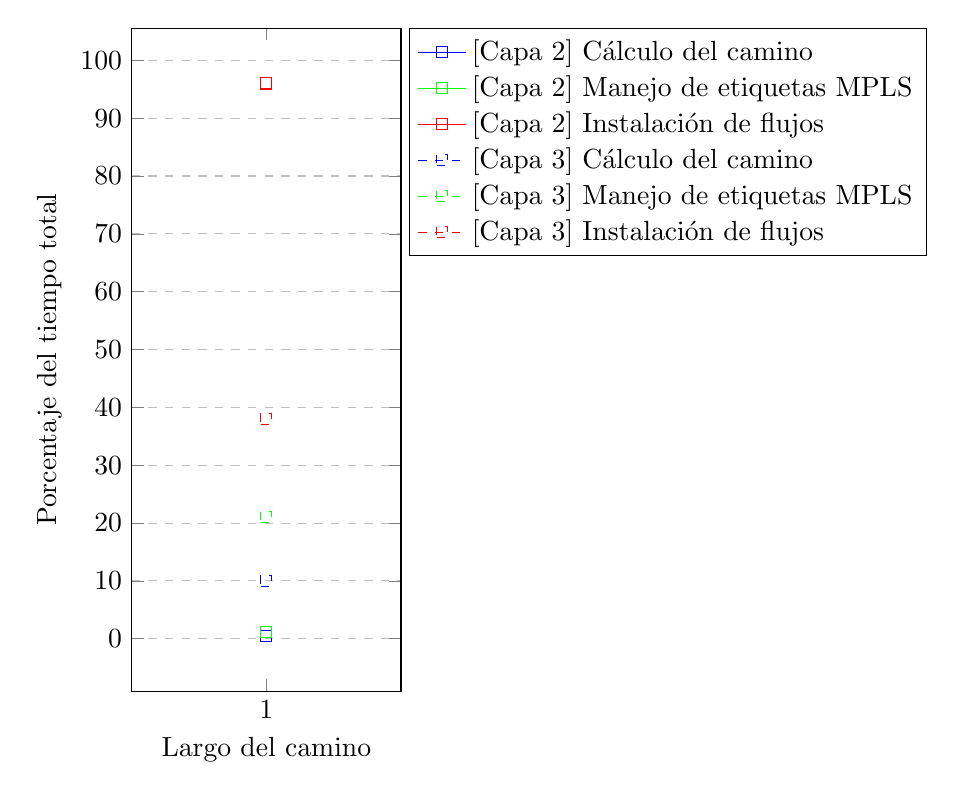
\begin{tikzpicture}
	\begin{axis}[
	xlabel={Largo del camino},
	ylabel={Porcentaje del tiempo total},
	xtick={0,1,2,4,6,8,10,12},
	ytick={0,10,20,30,40,50,60,70,80,90,100},
	scaled x ticks = false,
	x tick label style={/pgf/number format/fixed},
	legend pos= outer north east,
	ymajorgrids=true,
	grid style=dashed,
	width=5cm,
	height=10cm,
	legend cell align=left,
	]
	\addplot[
	color=blue,
	mark=square,
	]
	coordinates {
		(1,0.5)
	};
	\addlegendentry{[Capa 2] Cálculo del camino}
	\addplot[
	color=green,
	mark=square,
	]
	coordinates {
		(1,1.1)
	};
	\addlegendentry{[Capa 2] Manejo de etiquetas MPLS}
	\addplot[
	color=red,
	mark=square,
	]
	coordinates {
		(1,96)
	};
	\addlegendentry{[Capa 2] Instalación de flujos}
	\addplot[
	color=blue,
	mark=square,
	dashed,
	]
	coordinates {
		(1,10)
	};
	\addlegendentry{[Capa 3] Cálculo del camino}
	\addplot[
	color=green,
	mark=square,
	dashed,
	]
	coordinates {
		(1,21)
	};
	\addlegendentry{[Capa 3] Manejo de etiquetas MPLS}
	\addplot[
	color=red,
	mark=square,
	dashed,
	]
	coordinates {
		(1,38)
	};
	\addlegendentry{[Capa 3] Instalación de flujos}
	\end{axis}
	\end{tikzpicture}

	\caption{Distribución del tiempo de creación de VPNs en la topología chica}
	\centering
	\label{fig:gráfica_tiempo_chica}
	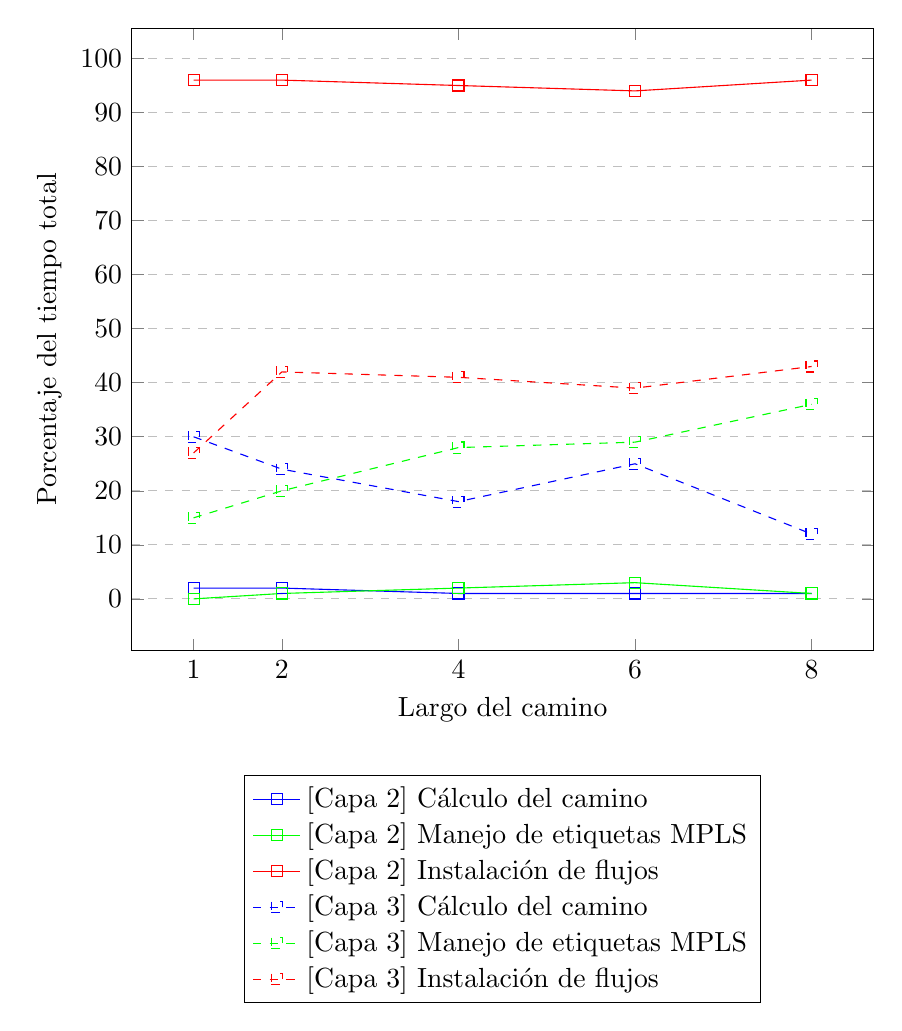
\begin{tikzpicture}
	\begin{axis}[
	xlabel={Largo del camino},
	ylabel={Porcentaje del tiempo total},
	xtick={0,1,2,4,6,8,10,12},
	ytick={0,10,20,30,40,50,60,70,80,90,100},
	scaled x ticks = false,
	x tick label style={/pgf/number format/fixed},
	legend style={at={(0.5,-0.2)},anchor=north},
	ymajorgrids=true,
	grid style=dashed,
	width=11cm,
	legend cell align=left,
	]
	\addplot[
	color=blue,
	mark=square,
	]
	coordinates {
		(1,2)(2,2)(4,1)(6,1)(8,1)
	};
	\addlegendentry{[Capa 2] Cálculo del camino}
	\addplot[
	color=green,
	mark=square,
	]
	coordinates {
		(1,0)(2,1)(4,2)(6,3)(8,1)
	};
	\addlegendentry{[Capa 2] Manejo de etiquetas MPLS}
	\addplot[
	color=red,
	mark=square,
	]
	coordinates {
		(1,96)(2,96)(4,95)(6,94)(8,96)
	};
	\addlegendentry{[Capa 2] Instalación de flujos}
	\addplot[
	color=blue,
	mark=square,
	dashed,
	]
	coordinates {
		(1,30)(2,24)(4,18)(6,25)(8,12)
	};
	\addlegendentry{[Capa 3] Cálculo del camino}
	\addplot[
	color=green,
	mark=square,
	dashed,
	]
	coordinates {
		(1,15)(2,20)(4,28)(6,29)(8,36)
	};
	\addlegendentry{[Capa 3] Manejo de etiquetas MPLS}
	\addplot[
	color=red,
	mark=square,
	dashed,
	]
	coordinates {
		(1,27)(2,42)(4,41)(6,39)(8,43)
	};
	\addlegendentry{[Capa 3] Instalación de flujos}
	\end{axis}
	\end{tikzpicture}
\end{figure}

\begin{figure}[H]
	\caption{Distribución del tiempo de creación de VPNs en la topología mediana}
	\centering
	\label{fig:gráfica_tiempo_mediana}
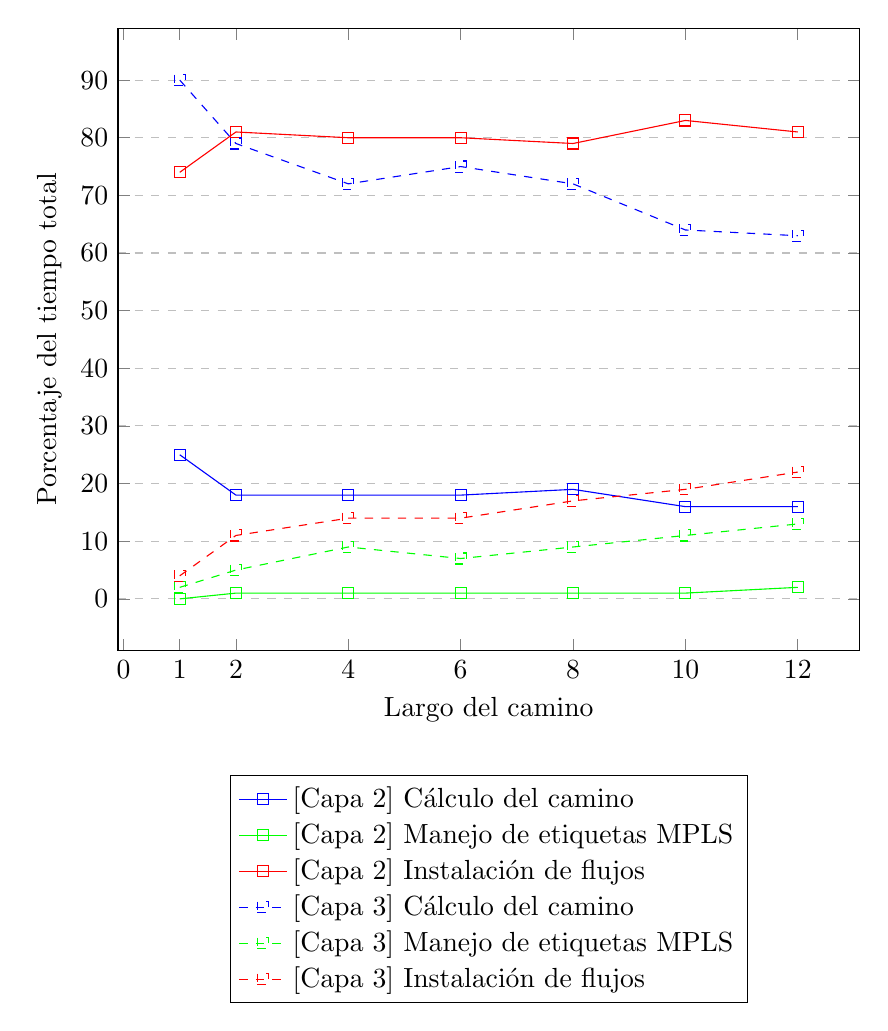
\begin{tikzpicture}
\begin{axis}[
xlabel={Largo del camino},
ylabel={Porcentaje del tiempo total},
xtick={0,1,2,4,6,8,10,12},
ytick={0,10,20,30,40,50,60,70,80,90,100},
scaled x ticks = false,
x tick label style={/pgf/number format/fixed},
legend style={at={(0.5,-0.2)},anchor=north},
ymajorgrids=true,
grid style=dashed,
width=11cm,
legend cell align=left,
]
\addplot[
color=blue,
mark=square,
]
coordinates {
	(1,25)(2,18)(4,18)(6,18)(8,19)(10,16)(12,16)
};
\addlegendentry{[Capa 2] Cálculo del camino}
\addplot[
color=green,
mark=square,
]
coordinates {
	(1,0)(2,1)(4,1)(6,1)(8,1)(10,1)(12,2)
};
\addlegendentry{[Capa 2] Manejo de etiquetas MPLS}
\addplot[
color=red,
mark=square,
]
coordinates {
	(1,74)(2,81)(4,80)(6,80)(8,79)(10,83)(12,81)
};
\addlegendentry{[Capa 2] Instalación de flujos}
\addplot[
color=blue,
mark=square,
dashed,
]
coordinates {
	(1,90)(2,79)(4,72)(6,75)(8,72)(10,64)(12,63)
};
\addlegendentry{[Capa 3] Cálculo del camino}
\addplot[
color=green,
mark=square,
dashed,
]
coordinates {
	(1,2)(2,5)(4,9)(6,7)(8,9)(10,11)(12,13)
};
\addlegendentry{[Capa 3] Manejo de etiquetas MPLS}
\addplot[
color=red,
mark=square,
dashed,
]
coordinates {
	(1,4)(2,11)(4,14)(6,14)(8,17)(10,19)(12,22)
};
\addlegendentry{[Capa 3] Instalación de flujos}
\end{axis}
\end{tikzpicture}
\end{figure}

\begin{figure}[H]
	\caption{Distribución del tiempo de creación de VPNs en la topología grande}
	\centering
	\label{fig:gráfica_tiempo_grande}
	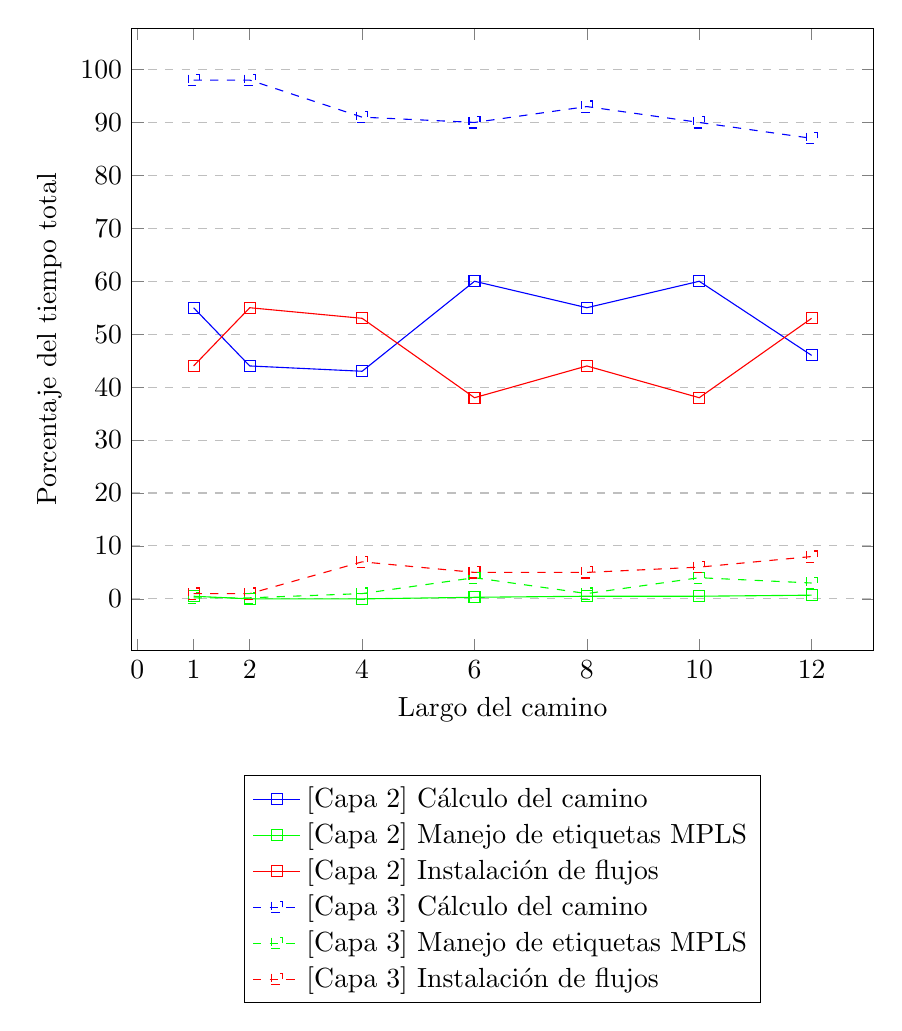
\begin{tikzpicture}
	\begin{axis}[
	xlabel={Largo del camino},
	ylabel={Porcentaje del tiempo total},
	xtick={0,1,2,4,6,8,10,12},
	ytick={0,10,20,30,40,50,60,70,80,90,100},
	scaled x ticks = false,
	x tick label style={/pgf/number format/fixed},
	legend style={at={(0.5,-0.2)},anchor=north},
	ymajorgrids=true,
	grid style=dashed,
	width=11cm,
	legend cell align=left,
	]
	\addplot[
	color=blue,
	mark=square,
	]
	coordinates {
		(1,55)(2,44)(4,43)(6,60)(8,55)(10,60)(12,46)
	};
	\addlegendentry{[Capa 2] Cálculo del camino}
	\addplot[
	color=green,
	mark=square,
	]
	coordinates {
		(1,0.5)(2,0)(4,0)(6,0.3)(8,0.5)(10,0.5)(12,0.7)
	};
	\addlegendentry{[Capa 2] Manejo de etiquetas MPLS}
	\addplot[
	color=red,
	mark=square,
	]
	coordinates {
		(1,44)(2,55)(4,53)(6,38)(8,44)(10,38)(12,53)
	};
	\addlegendentry{[Capa 2] Instalación de flujos}
	\addplot[
	color=blue,
	mark=square,
	dashed,
	]
	coordinates {
		(1,98)(2,98)(4,91)(6,90)(8,93)(10,90)(12,87)
	};
	\addlegendentry{[Capa 3] Cálculo del camino}
	\addplot[
	color=green,
	mark=square,
	dashed,
	]
	coordinates {
		(1,0.2)(2,0.2)(4,1)(6,4)(8,1)(10,4)(12,3)
	};
	\addlegendentry{[Capa 3] Manejo de etiquetas MPLS}
	\addplot[
	color=red,
	mark=square,
	dashed,
	]
	coordinates {
		(1,1)(2,1)(4,7)(6,5)(8,5)(10,6)(12,8)
	};
	\addlegendentry{[Capa 3] Instalación de flujos}
	\end{axis}
	\end{tikzpicture}
\end{figure}

**Algunas conclusiones de estos resultados.


\section{Escala de servicios y flujos}
Entre los requerimientos de la RAU2 se encuentra el de la escalabilidad de usuarios. En particular, se espera alcanzar en un mediano plazo un total de 11.000 docentes, 7.000 funcionarios y 140.000 estudiantes (de acuerdo a los requerimientos relevados por el proyecto RRAP). Esto implica que la red será sujeta a importantes cantidades de servicios y flujos distintos. He aquí la relevancia de las pruebas en la presente sección. Mediante el entorno virtual, se someterá la arquitectura a una cantidad de servicios relativamente grande y de esta forma se podrían identificar posibles puntos de falla, o umbrales bajo los cuales debe mantenerse la red para funcionar con buen rendimiento. Es importante recordar que aunque el entorno de simulación permite hacer un valioso estudio de escalabilidad, no generará resultados relevantes en lo que refiere al nivel real de rendimiento de la arquitectura. Recordar sección 3.3.1, donde se explica que cada instancia de Open vSwitch se ejecuta en modo user-space, y por ende procesa los paquetes de forma bastante lenta.

\subsection{Descripción del escenario}
La idea principal del escenario es crear muchas VPN y analizar los comportamientos que esto genera. Se utiliza una VPN punto a punto de capa 3 para conectar dos subredes cliente, y se utiliza \textit{iperf} para generar tráfico TCP y medir el ancho de banda entre los dos RAUHost. Para cargar a la arquitectura con servicios, se crean múltiples VPN de capa 2 entre las subredes, variando los valores de los cabezales VLAN\_ID y VLAN\_PCP (pudiendo crear un total de 32.768 combinaciones distintas) para que toda VPN sea distinta de las demás. De esta forma, existirán múltiples VPN pero solo una (la de capa 3) será utilizada. \\
Dado que cargar todas las VPN a mano en la interfaz web llevaría demasiado tiempo, se creó un servicio web que recibe como parámetro la cantidad de VPN que se desean. Cuando se hace un pedido GET a ese servicio web, se inicia el proceso de creación de las mismas. Este proceso puede tomar entre algunos minutos y varias horas, dependiendo de la cantidad. \\ \\
El objetivo es verificar los siguientes dos aspectos claves: \\ \\
\textbf{Escalabilidad interna del RAUSwitch} \\
Se estudian posibles limitaciones internas que puedan tener los dispositivos, cuando deben manejar grandes cantidades de flujos. Es posible que a medida que crece su tabla de flujos, demoren más en encontrar el flujo que se corresponde con cada paquete que reciben. Si pasa esto, el throughput debería ser afectado negativamente por la cantidad de flujos en sus tablas. Se utilizará \textit{iperf} para medir la velocidad de transferencia entre las subredes cliente.  \\ \\
\textbf{Escalabilidad en servicios} \\
Se estudian posibles problemas que puedan tener la arquitectura de la red o, en particular, la aplicación RAUFlow para manejar grandes cantidades de servicios o información. Es de particular interés medir la memoria que requiere el controlador para mantener los servicios. \\ \\
Esta prueba se repite para las mismas topologias que la prueba anterior, es decir: básica (4 nodos), chica (11 nodos) y mediana (45 nodos).

\subsection{Resultados y observaciones}

\begin{table}[ht]
	\caption{Throughput en Kbits/s para cada caso.}
	\centering 
	\begin{tabular}{c c c c c}
		\hline\hline
		\# de VPN & Básica & Chica & Mediana  & Grande \\ [0.5ex]
		\hline
		1 & 893 & Y & W & Z \\
		3000 & 887 & Y & W & Z  \\
		6000 & 887 & Y & W & Z \\
		9000 & 890 & Y & W & Z \\
		12000 & 885 & Y & W & Z \\
		15000 & 886 & Y & W & Z \\ [1ex]
		\hline
	\end{tabular}
	\label{table:escala_de_servicios}
\end{table}

Como se explica en el primer objetivo de esta prueba, se busca determinar si la existencia de muchos flujos en la tabla, implica que un switch OpenFlow demora más tiempo en encontrar el flujo que corresponde para un paquete entrante, y por lo tanto demora más en determinar la acción a tomar para ese paquete. Si esto fuera así, debería existir una relación inversamente proporcional entre la cantidad de flujos en la tabla de un nodo y su velocidad para procesar paquetes. En la tabla \ref{table:escala_de_servicios} se pueden observar los throughput promedio medidos para un flujo de datos sobre la topología básica, con distintas cantidades de VPN existiendo en la red. La principal conclusión que se puede sacar de la tabla es que el throughput es constante para un camino y topología, sin importar la cantidad de VPN existentes en el momento (se asume que las pequeñas diferencias numéricas entran en el margen de error). \\
La máxima cantidad de VPN con la que se probó fue de 15.000. Cada VPN de capa 2 está compuesta por dos servicios de capa 2, y cada uno de esos servicios introduce 42 flujos en cada nodo del camino. Esto quiere decir que cada uno contiene alrededor de 1.260.000 (15.000 * 2 * 42) flujos en su tabla. Se podría argumentar que hacen falta más flujos para impactar el throughput, pero en realidad la explicación de porqué esa cantidad de flujos no afecta se encuentra en la especificación de Open vSwitch, y ya fue mencionada en el capítulo 3. Open vSwitch realiza cacheo de flujos. Eso quiere decir que cuando un paquete de datos de un determinado flujo llega por primera vez a un nodo, este paquete es enviado al pipeline de OpenFlow para determinar qué acción se debe tomar. Luego de realizada, esta acción es escrita en la caché, y tiene un tiempo de vida de entre 5 y 10 segundos. Si en ese período de tiempo llega otro paquete del mismo flujo, no hay necesidad de enviar el paquete al pipeline, porque ya se sabe cuales son las acciones a tomar para el mismo. Por lo tanto, si un flujo de datos es constante y rápido, el tamaño de la tabla de OpenFlow no afectará el tiempo de decisión, ya que sólo el primer paquete de ese flujo deberá ser comparado con dicha tabla.

Mediante el comando 'ovs-appctl dpctl/show' de Open vSwitch, se puede examinar las estadísticas de la cache de cada nodo. A modo de ejemplo, en la figura \ref{fig:cache_sample} se observan las estadísticas de un nodo llamado 'alice'. En la sección 'lookups' se detallan cuantos 'hits' y 'miss' de caché han ocurrido hasta el momento, y 'flows' indica cuantos flujos activos hay en el momento en la caché.

\begin{figure}[H]
	\caption{Estadísticas de cache de flujos del nodo 'alice'.}
	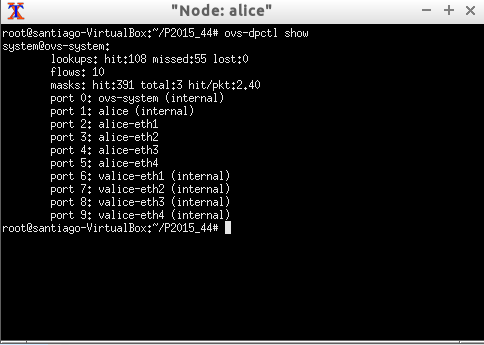
\includegraphics[scale=1]{cache_sample}
	\centering
	\label{fig:cache_sample}
\end{figure}

Otro objetivo de la prueba es determinar si la arquitectura, y en particular el controlador, tienen algún problema para manejar muchos servicios. En la prueba de servicios ya mencionada no se detectó ningún problema de esa índole. Sin embargo, es importante recordar que el controlador mantiene toda su información en memoria, por lo tanto es de interés realizar un estudio del consumo de memoria del mismo a medida que crece la cantidad de servicios. El comando de Linux llamado \textit{pmap} permite estudiar el consumo de memoria del proceso que se le indique, y con el mismo podemos analizar la evolución del consumo de memoria del controlador a medida que se le agregan servicios. En la tabla \ref{table:consumo_de_memoria} y la siguiente gráfica se puede observar el resultado de estas mediciones. \\

\begin{table}[ht]
	\caption{Evolución del consumo de memoria del controlador.}
	\centering 
	\begin{tabular}{c c}
		\hline\hline
		Cantidad de VPN & Memoria (KB) \\ [0.5ex]
		\hline
		0 & 33280 \\
		3000 & 108196 \\
		6000 & 182460 \\
		9000 & 256528 \\
		12000 & 333244 \\
		15000 & 407696 \\ [1ex]
		\hline
	\end{tabular}
	\label{table:consumo_de_memoria}
\end{table}

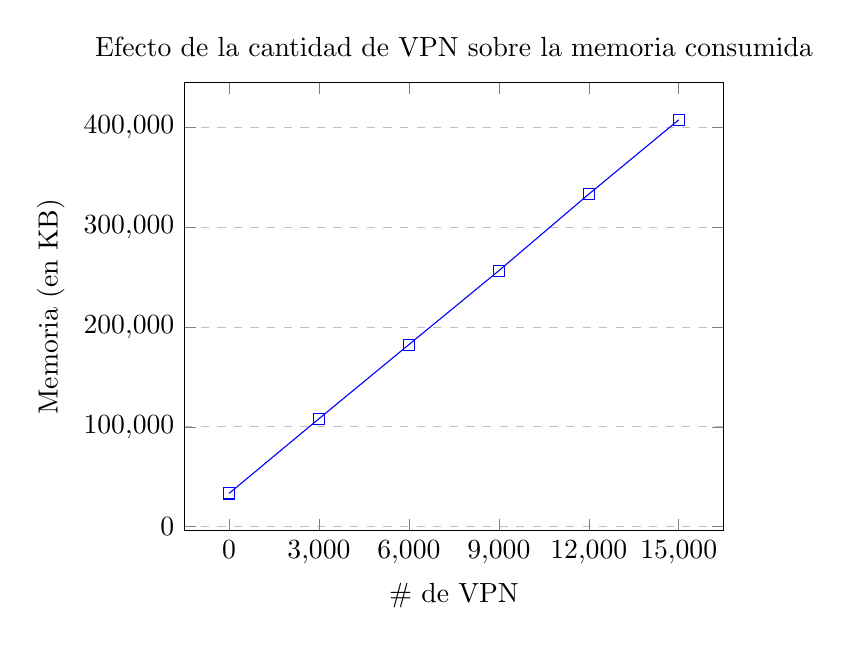
\begin{tikzpicture}
\begin{axis}[
title={Efecto de la cantidad de VPN sobre la memoria consumida},
xlabel={\# de VPN},
ylabel={Memoria (en KB)},
xtick={0,3000,6000,9000,12000,15000},
ytick={0,100000,200000,300000,400000,500000},
scaled x ticks = false,
scaled y ticks = false,
x tick label style={/pgf/number format/fixed},
y tick label style={/pgf/number format/fixed},
legend pos=north west,
ymajorgrids=true,
grid style=dashed,
]
\addplot[
color=blue,
mark=square,
]
coordinates {
	(0,33280)(3000,108196)(6000,182460)(9000,256528)(12000,333244)(15000,407696)
};
\end{axis}
\end{tikzpicture}

La principal observación que se puede hacer es que el consumo de memoria del controlador aumenta de forma lineal con la cantidad de servicios. El mismo se incrementa en 74916 KB cada 3000 servicios, por lo tanto se puede calcular que cada servicio ocupa alrededor de 25 KB (74916/3000). A modo de ejemplo, si extrapolamos ese número a una computadora que puede dedicar 4 Gb de RAM para mantener los servicios, llegamos a que el controlador podrá mantener alrededor de 167.772 servicios. A pesar de que no es ideal mantener tantos datos en memoria, se puede concluir que es un consumo aceptable. \\

En el proceso de realizar las pruebas ya mencionadas también se observó un comportamiento que no se esperaba. Se detectó que a medida que hay más VPN creadas, la red demora más tiempo en crear una nueva VPN. Con el propósito de entender más ese comportamiento, se hizo un experimento cuyos resultados se observan en la siguiente gráfica. \\ \\
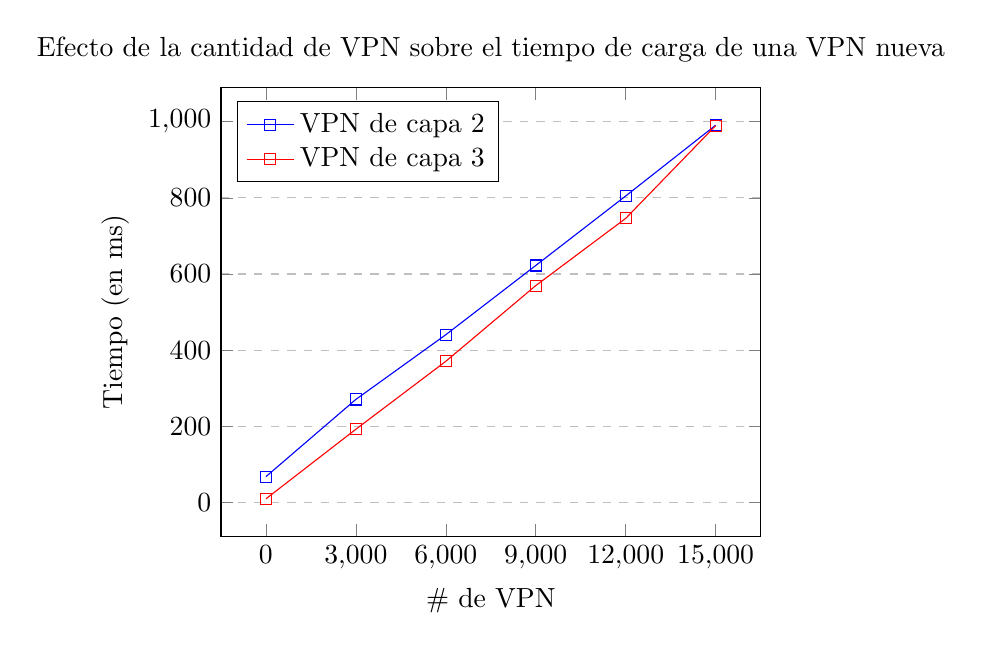
\begin{tikzpicture}
\begin{axis}[
title={Efecto de la cantidad de VPN sobre el tiempo de carga de una VPN nueva},
xlabel={\# de VPN},
ylabel={Tiempo (en ms)},
xtick={0,3000,6000,9000,12000,15000},
ytick={0,200,400,600,800,1000,1200},
scaled x ticks = false,
x tick label style={/pgf/number format/fixed},
legend pos=north west,
ymajorgrids=true,
grid style=dashed,
]
\addplot[
color=blue,
mark=square,
]
coordinates {
	(1,68.2)(3000,270.9)(6000,440.7)(9000,622.4)(12000,804.8)(15000,990.5)
};
\addlegendentry{VPN de capa 2}
\addplot[
color=red,
mark=square,
]
coordinates {
	(1,10.0)(3000,192.6)(6000,370.9)(9000,569.6)(12000,746.0)(15000,989.3)
};
\addlegendentry{VPN de capa 3}
\end{axis}
\end{tikzpicture}

Cada punto indica el tiempo que demora la red en dar de alta una nueva VPN con una determinada cantidad de VPN ya existentes. Estos tiempos se miden de la misma forma que los obtenidos en la sección de pruebas anterior: se toma el tiempo que demora la aplicación en devolver la respuesta HTTP indicando que el servicio se creó con éxito (disponible en los logs). En la gráfica se puede ver que el tiempo de carga aumenta de forma lineal a medida que hay más VPN en la red, y esto se cumple para la de capa 2 como la de capa 3. Una posible explicación inicial para esto puede ser que al tener más flujos, cada nodo demora más en insertar nuevos flujos en su tabla. Esa teoría se descarta con el siguiente razonamiento. En la gráfica se observa que toma más tiempo crear una VPN de capa 2 que una de capa 3. Esto en gran medida se explica porque un servicio de capa 2 debe insertar 42 flujos en los nodos del camino, mientras que uno de capa 3 solo inserta 1. Pero también se observa que las lineas son virtualmente paralelas, es decir, esa diferencia de tiempo se mantiene constante a pesar de las VPN que existan. Si insertar un flujo nuevo cada vez tomara más tiempo, ese incremento se debería multiplicar por 42 para la VPN de capa 2, y la linea correspondiente a la VPN de capa 2 debería tener una pendiente más inclinada que la de capa 3. \\
Otra posible explicación para este comportamiento puede ser que la aplicación RAUFlow se vuelve más lenta a medida que sus estructuras de datos crecen. Sin embargo, no se observó ningún patrón en el código que indique esto. \\ \\

***Algunas conclusiones de estas pruebas.